\documentclass[a4paper, 11pt]{kth-mag}
\usepackage[T1]{fontenc}
\usepackage{textcomp}
\usepackage{lmodern}
\usepackage[latin1]{inputenc}
\usepackage[swedish,english]{babel}
\usepackage{modifications}
\usepackage{listings}
 \usepackage{graphicx}
\title{Stress Tetris}

\subtitle{Is it Possible to Manipulate EDA (Electrodermal Activity)?}
\foreigntitle{Stress-tetris - g�r det att manipulera EDA (Electrodermal Activity)?}
\author{Martin Pettersson\\Daniel Swensson}
\date{April 2013}
\blurb{Bachelor's Thesis at KTH CSC\\Supervisor: Anna Hjalmarsson}

\begin{document}
\frontmatter
\pagestyle{empty}
\removepagenumbers
\maketitle
\selectlanguage{english}
\begin{abstract}
The idea behind this project was to implement and study biofeedback features in the popular video game Tetris, using EDA (Electrodermal activity). The goal was to explore if it is possible to deliberately alter live EDA measurements using a Q-Sensor wristband along with the game. Our implementation can change the speed of the game according to the current EDA value of the player. The problem was studied by issuing a user test experiment along with a survey questioning how test subjects responded to the biofeedback features. Results showed that manipulating EDA in our version of Tetris seem possible, although subjects could only alter EDA for shorter periods of time rather than manipulating a general value. However, the results obtained are contradictory in several aspects and more research is needed to make these more explicit.

More accurate results would require more work and knowledge than presented in this study.
\end{abstract}
\clearpage
\begin{foreignabstract}{swedish}
Tanken bakom detta projekt var att implementera och studera biofeedback-element i det popul�ra datorspelet Tetris genom att anv�nda EDA (Electrodermal activity). M�let var att unders�ka om det �r m�jligt att medvetet manipulera EDA-m�tningar vid anv�ndandet av ett Q-Sensor-armband tillsammans med spelet. V�r implementation kan �ndra spelets hastighet beroende p� vilket EDA-v�rde en spelare vid tillf�llet har. Problemet studerades genom att utf�ra ett anv�ndartest tillsammans med en fr�ge-enk�t f�r att unders�ka hur testpersoner svarade till biofeedback-elementen. Resultaten visade att det kan vara m�jligt att medvetet manipulera EDA-m�tningar vid spelande av Tetris, dock kunde f�rs�kspersonerna bara f�r�ndra dessa m�tningar under kortare perioder snarare �n att p�verka genomsnittsv�rdet. Resultaten �r mots�gelsefulla p� m�nga punkter och mer forskning i �mnet �r n�dv�ndigt f�r att dessa ska bli mer tydliga.

Mer tillf�rlitliga resultat kr�ver betydligt mer arbete och kunskap �n vad som framst�lls i denna rapport.
\end{foreignabstract}
\clearpage
\tableofcontents*
\mainmatter

\chapter{Introduction}

Electrodermal activity (EDA) measurements are forms of technologies developed to measure sweat levels in human skin. "For most people, if one experiences emotional arousal, increased cognitive workload or physical exertion, the brain sends signals to the skin in order to increase the level of sweating." \cite{affectiva}

EDA is interesting to use for measurement of cognitive activity during specific objectives or tasks, such as analysing emotional differences between an experienced car driver and someone who uses a car for the very first time with no prior experience. \cite{driving}

Some research combining live EDA streaming and commercial computer game titles have been made. Most of these implementations have been modified titles in the First Person Shooter-genre (FPS). \cite{fps} So far, research made on enhanced computer game mechanics using EDA biofeedback has been relatively unexplored.

A study from 2010 \cite{tetris10} focused on finding an optimal state of mind while playing a game of the classical computer game Tetris. The study stated that while a computer game generally is intended to affect the player in a positive way (such as positive excitement), it may however impact the player in a more diverse manner, largely depending on the difficulty of the game. It was suggested that players became more negatively affected if the difficulty was too hard or too easy, with emotions ranging from boredom to frustration. The idea was to calm the player when feeling stressed and induce excitement during states of boredom, thus forcing the game to adapt its difficulty to the player and make the experience more positive and exciting. The same article proposed demonstration techniques but mentions no concrete results of these experiments.

With this study we wanted to explore these ideas further but with a slightly different approach, focusing on stressful situations. The Tetris implementation in the report from 2010 made the game easier when a player became emotionally aroused or stressed and increased the difficulty during calmness. We implemented a similar version of the game, but with opposite biofeedback functionality, letting the game speed increase when a player became stressed. The reason for this choice was to determine if players could deliberately alter their EDA value. With a user experiment we tested this by letting several test subjects play our own EDA version of Tetris while trying to make the game go faster and slower on demand.

\section{Statement of Collaboration}
The implementation of EDA feedback along with the Tetris game, written in Java and included in the appendix is a product of Daniel Swensson. Swensson also initiated and made the study visit to SICS (The Swedish Institute of Computer Science) and executed the user experiment. The bulk of the report was written by Martin Pettersson, who also had contact with the supervisor and scheduled borrowing of the Q-Sensor wristband. Data plots, experimental results analysis and proof reading were all outcomes of collaborative work between both parts.

\section{Problem Statement}
This study was performed with the intention of exploring the possibility of user test subjects deliberately controlling or manipulating live measurements of electrodermal activity when confronted with a task that produces some levels of stress and arousal. More specifically, the task performed was a play session of the classic computer game Tetris, modified to change game speed according to live recordings of EDA data using a Q-Sensor device. The study poses the question if players could deliberately change the game speed themselves. 

The problem stated is interesting for several reasons, where we may present a few. One reason may be when EDA is used in relation to computer gaming, where it is highly relevant since manipulating live measurements of EDA may change states and game mechanics of such games and thus making biofeedback game elements favorable for players who are good at controlling their stress levels. Although controversial, live measurements of EDA have been used in various types of lie detecting systems. If subjects confronted with such systems have the possibility of manipulating EDA that would further question the credibility of EDA-based polygraph technology. 

\section{Limitations}
Although the problem this study was intended to explore was stated in a general manner, many limitations were introduced mainly due to time and budget constraints. The measurement of electrodermal activity is solely limited to what the equipment, in this case a modified Affectiva Q-Sensor, can perform. The limitations of the sensor wristband are explained further in the background section. One could argue that a study like this should explore a broad spectrum of stressful tasks for subjects to confront, however time constraints limited us to focus solely on the Tetris implementation.

Another constraint is that of the user experiment, which was limited to include only a handful of test subjects.

With these issues in mind, the reader should observe the results and conclusions made from the study in a critical manner, and further studies of the problem are needed in order to give a more convincing result. A section regarding suggestions for further study on the subject is devoted under the discussion section of the report.


\chapter{Background}

\section{Electrodermal Activity}
Research has shown that when a majority of people experiences emotional arousal or physical exertion, or increases their cognitive workload, the brain signals the skin to produce more sweat. One may not actually feel the increased amount of sweat levels or even feel any sort of difference in sweating at all. However, the greatest difference is that of the change in electrical conductance of the skin, which is actually increased significantly when most people endure stressful situations or increase cognitive workload. This change in electrical conductance is due to salt water (sweat) that more gradually fills up pores beneath the skin.

Electrodermal activity, often abbreviated just EDA, is a term that refers to electrical changes on the surface of the skin as the brain sends signals in order to increase the amount of sweating on that particular area. \cite{affectiva}

There are various methods available for measurements of a person's electrodermal activity. These ways in which EDA can be measured are often divided into two categories, including endosomatic measurements and exosomatic measurements.

\begin{itemize}
  \item Endosomatic measurements: A technique that involves microneurography, where electrodes are placed directly onto the skin's neurons.
  \item Exosomatic measurements: Here measurements are executed by placing two external electrodes onto the surface of the skin. An electrical current of very low magnitude is sent between the electrodes and the skin surface.
\end{itemize}

The measurement of EDA values is interesting for several reasons, such as analysing the difference between an experienced car driver and a subject who uses a car for the first time. Another field of interest where these measurements are used is in the study of creating new systems for polygraphy, more commonly known as lie detectors.

Another more unexplored field is the use of live EDA measurements for direct biofeedback in various tasks, such as computer games \cite{fps, tetris10}. It is this field the report will mostly focus on.

\section{The Tetris Game}
This block matching puzzle game was originally published in 1984 by Russian mathematician Alexey Payitnov, and became by far the most popular video game ever to be released by the USSR. The legacy of the game holds strong still to this date, and almost everyone will come across it at some point.

For the oblivious reader, the report will make a short introduction of the game rules.

In Tetris, the set of all 4-polyminoes (tetriminoes), keeps being pulled down by a gravitational constant in a vertical play field. It is up to the player to arrange theese falling blocks so that they line up in perfect rows, without "holes". If a perfect row is arranged, that row disappears from the play field and the player is rewarded with score points. The player gains more score points depending on how many perfect lines he or she can create at the same time. The maximal clearing situation occurs when the player assembles four perfect lines at the same time, giving a perfect score. This situation is referred to as a "Tetris". The game ends when the entire vertical play field is filled and no more blocks longer can fit or fall down. The object of the player is to survive long enough and gain as many score points as possible. A game session is often accompanied by traditional Russian folk tunes.

The game was a good choice for the experimental setup for this study, mainly because the game is easy enough to grasp, induces some moderate stress to players, and is relatively simple to modify in terms of changing difficulty settings, game speed, etc.

\section{The Affectiva Q-Sensor}
Affectiva, a company producing branded EDA sensor wristbands, describes their Q-Sensor as a wearable, wireless biosensor that measures emotional arousal via skin conductance, a form of electrodermal activity. In case of this study, the device was slightly modified in order for the electrodes to be wearable at the tip of the fingers instead of the wrist. The reason for this is that conductance that correlates to EDA seems to be more significant when measured on fingertips rather than on wrists, which is a newer measurement method according to Affectiva. With such a device one may implement biofeedback features in interactive software as well as record EDA values simultaneously.

\begin{figure}
\centerline{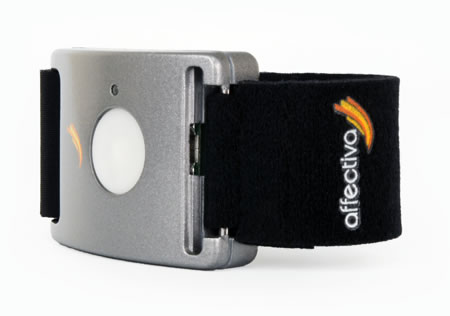
\includegraphics[scale = 3]{sensor.jpg}}
\caption{The Affectiva Q-Sensor. \cite{affectiva}}
\end{figure}

The main reason choosing this kind of sensor in a study like this one is because of the ease to stream recorded data live via the Bluetooth protocol, which makes the device ideal for live EDA biofeedback in computer games or similar interactive software. Another benefit is how convenient the wristband is to wear; no other equipment is required for it to work, a subject simply needs to wear the wristband and it will automatically record and stream EDA data with very few external requirements. \cite{affectiva}

\section{Study Visit at SICS}
The Swedish Institute of Computer Science is an independent and non-profit research organisation with a main interest of research in computer science. It came to our knowledge that the institute had made some research on EDA, and that they had knowledge of similar devices to the Q-Sensor. After some initial contact we were invited to their main office in Kista by Johanna Mercurio, who works as a researcher and project manager at SICS's Mobile Life Center division. The main purpose of the visit was to discuss our thesis and gain more knowledge about what capabilities sensors measuring EDA has had in their research projects.

The institute's most noticeable research project regarding EDA has been the development of a Smartphone application that uses live EDA measurement data from a sensor wristband. \cite{sics} The application logs and synchronises data obtained from a wristband, and then presents these data to a user in a visually engaging and pleasing way. The wristband itself was not an Affectiva Q-Sensor, but a similar device hand crafted by Philips Corp. and produced solely for research purposes. According to Mercurio, the main purpose of the project was not to further research electrodermal activity, focus was more shifted towards human-computer interaction-related fields. The bulk of their work was concentrated on visual representation and design elements. 

With this application the division has issued a number of user experiments. Mercurio mentioned one experiment in particular where a research team had provided the application to elite orienteering sportsmen. The purpose of the experiment was to study if these sportsmen improved their skills upon realisation of their stress magnitudes and levels of arousal. Mercurio could not provide more information regarding the results, but mentioned that reactions to the experiment so far have been very positive. She also stated that they believed EDA wristbands to be a promising successor to popular commercial pulse monitors often used in sport contexts, as EDA provided more interesting data in comparison.

When asked about our thesis, regarding whether it is possible for users of similar wristbands to purposefully manipulate and change EDA values, she stated that she has not yet been aware of any successful attempts of users changing the average value. However, Mercurio knew for certain that a user could change values temporary by for instance overbreathing or taking very deep breaths. She said that it is very plausible that a deliberate change in focus of a wristband user could cause measurement changes, but that it wasn't something the institute had researched. Suddenly making wristband users startled or frightened produces short but significant changes in measurements.

\chapter{Method}
The realisation of this study came to include two different elements: the implementation of the EDA biofeedback features in a Tetris clone, and a user test experiment.

\section{Implementation}

\begin{lstlisting}[language=java]

\end{lstlisting}

\subsection{Approach}
Our initial idea on how to implement live EDA biofeedback in Tetris was stated in the project specification, as follows:

"Starting off, the first implementation of the game will only change the game speed depending on EDA biofeedback signals. This implementation will be tested before the actual study is issued. If measurement data from this version proves to be insufficient or unsecure (for instance, the subject never gets stressed out), we may introduce "elements of surprise" during calmness in order to force the player to become more aroused. Examples of such surprise elements may be that game controls suddenly becomes reversed, Tetrimino blocks switches to another block in mid-air, or introducing time limit elements (such as to fill a row in a short period of time)."

Due to time constraints and the general difficulty of developing a full size Tetris clone, we decided early on to modify the EDA biofeedback speed element to an already existing open source version of the game. 

\subsubsection{Choice of platform and Tetris version}
We decided to develop for the Windows platform early on, mostly because we didn't have any other suitable and portable system for developing available that could run another system.

After some initial research of potential Tetris clones we could modify, we found source code for two open source versions of the game. One was written in C and the other one in Java. \cite{code} Even though we realised that the version written in C had a better design and was more enjoyable to play, we decided to modify the Java clone since we both were more proficient in the language. Another profit gained from choosing Java instead of C was more ease in compilation. 

\subsubsection{Methods for changing game speed}
One crucial element of the game was to be able to change the speed of the game when the Q-Sensor device reacted to EDA from a user. In the project specification we stated that we wanted the game to go faster when EDA measurements went up, and slower when the values decreased. We proposed following methods in order to do this:


\begin{enumerate}
  \item Begin by measure the player's average EDA before the game session during a short period of time in order to calibrate the initial speed of the game. Thereafter we would change the speed directly according to current EDA values.
  \item Measure EDA values continuously during even time intervals and calculate the average value of one period, and then set the game speed according to that average value.
  \item Like the previous method, only that we compare the current EDA average value with that of the previous time interval. However, the game changes speed according to a constant value.
\end{enumerate}

After some discussion with other project groups also focusing on Q-Sensors, we decided to use the interval method (number 3 in the list above), with intervals of five seconds in duration, and with constant change of game speed for improved playability. The main reason for choosing this method was that it gave more reliable measurement data and made it easier to compare data between subjects and groups for given time intervals. This method turned out to be good because we were able to see if a subject was more aroused in a particular moment in time compared to the previous time interval.

\subsubsection{Bluetooth communication}
The Affectiva Q-Sensor uses a virtual Bluetooth serial port for communication. On the Windows platform this appears as a numbered COM-port. Via this protocol, the device streams unencrypted messages live in plain text, according to the example below:

\centerline{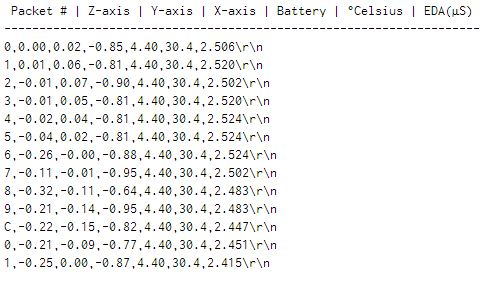
\includegraphics{kod1.JPG}}

At this moment Java no longer has any active libraries to use for reading serial COM-ports on the Windows platform. After some tests of third party libraries, we finally chose RXTX \cite{r} to be most suitable for our needs.

In RXTX, the SerialPortEventListener class detects when there are byte data available in the port stream and reads one message line at a time, and then stops at a newline character. Byte data are then converted and stored as a string for further use:

\centerline{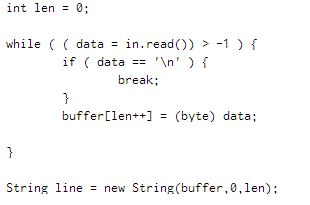
\includegraphics{kod2.JPG}}

\subsubsection{Comparing a median EDA value over a set of time intervals}
When reading each line the message is split to easily pick out the EDA value. The value is then converted from String to float and stored in the ArrayList labeled m.

The Q-Sensor was set to measure at 32 Hz. Thus we set a constant, freq, to 32 * 5 = 160 as the number of measurements during a 5 second interval. This was later halved to 80 (2,5 seconds) to improve playability and to make the game more responsive.

The constant was also raised to 81, an odd number, to avoid extra operations when calculating the median EDA value.

When the number of read lines reaches 81 the median of all the measurement values in the ArrayList is calculated and compared to the median of the last 2,5 second interval.

The Boolean labeled increased, is set depending if there is an increase during the comparison or not. The Boolean labeled ready is set to true as a flag to signal the Tetris game when a new interval has been measured and calculated. These two Boolean variables are accessible by the game via public methods.
\begin{figure}
\centerline{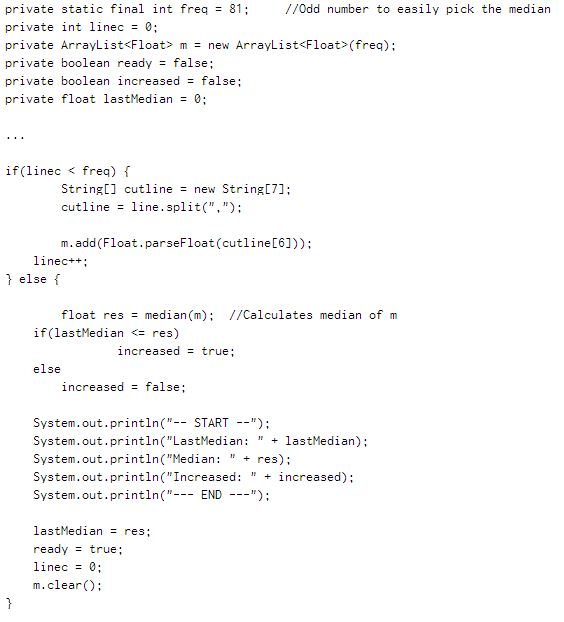
\includegraphics{kod3.JPG}}
\caption{As described in previous section.}
\end{figure}
\begin{figure}
\centerline{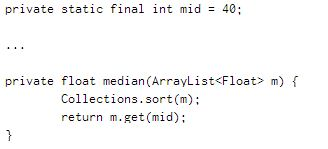
\includegraphics{kod4.JPG}}
\caption{Calculating the median value.}
\end{figure}
\begin{figure}
\centerline{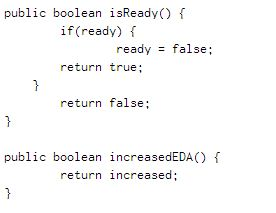
\includegraphics{kod5.JPG}}
\caption{Public methods for communication with the Tetris class.}
\end{figure}

\subsubsection{Modifying the game speed}
After examining the Java source code of the Tetris game we noticed that the game speed was raised with a small constant every time a block was dropped. We used this to our advantage to further improve playability.

Whenever a block was dropped we checked if the measured interval median had changed and raised or lowered the game speed by a larger constant. Only changing the speed when the block was dropped gave the player more control. Knowing when the speed was going to change gave the player an opportunity to try to manipulate their EDA-level.

The old speed change code was modified to call serialComm.isReady() and serialComm.increasedEDA() to check if the measurements had increased or decreased within the last 2,5 seconds and add or subtract the SPEEDCHANGE constant to the gameSpeed variable accordingly.

We also added initialisation of the PortReader class in order to start reading from the Q-Sensor when the game is loading.

Prior to the experiment we tested the modified game on a test subject not included in the experiment. After the test we added a maximum speed limit and adjusted the constant of speed change in order to not make the game too hard for inexperienced Tetris players but still induce a noticeable change in speed. 

\begin{figure}
\centerline{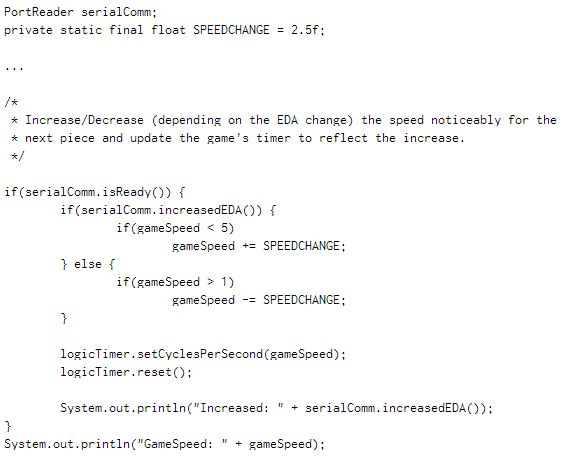
\includegraphics{kod6.JPG}}
\caption{Speed modifications.}
\end{figure}
\begin{figure}
\centerline{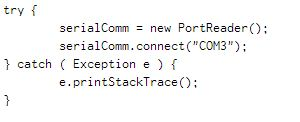
\includegraphics{kod7.JPG}}
\caption{Initialisation of the port reader.}
\end{figure}

\subsection{Problems}
Being inexperienced with reading from a virtual serial port the first problem that arose was finding a currently maintained and working Java library for that purpose. At first we used the official javax.comm.CommPort but it turned out to be outdated (not working as intended in recent versions of Windows) and no longer supported by Oracle.

Then we tried jSSC (Java Simple Serial Connector) and managed to read raw byte stream data from the Q-Sensor. However a second major problem appeared. We could not parse separate message lines reliably using byte offsets.

After a long session of debugging it turned out that the some messages were of different length. This was because the XYZ-values from the accelerometer in the sensor could appear as negative and add a subtraction symbol prior to the message line. 

This was finally solved by switching to the RXTX-library, using an EventListener and reading until reaching a newline character.
\subsection{Final Version}
The final modified Tetris game used during the experiment has three different constant speed levels which it can switch between when a Tetrimino block drops. This differs from what we intended from the beginning when we just wanted the speed to directly correlate to the EDA value. Reading from the Q-Sensor and the calculations in the background were also not anticipated because of the same reason.

The speed change is visible by looking at the level indicator on the game interface and also the speed is changing with a large enough constant that it�s noticeable just by looking at the blocks while playing.

The game is controlled with only one hand and has, even without the Q-Sensor, slightly unconventional controls and game mechanics. This combined with the high speed changes throws off even experienced Tetris players, making the game more stressful than we anticipated. 

The �elements of surprise� were not needed, opposite to our prior beliefs.

\section{User Experiment}
In order to arrive at any conclusions for the problem stated, a quantitative user experiment was issued along with a survey of some questions regarding the experiment. The general idea behind this was to divide test users into two groups given different instructions. One group served to test the problem statement directly (is it possible to deliberately manipulate EDA?) and another group served as reference. With data provided from both groups the intention was to make a simple statistical comparison between them and from there discuss results and arrive at proper conclusions.

\subsection{Approach}
The user experiment was issued by letting both groups of test subjects play the EDA biofeedback Tetris implementation for a five minute duration. Each group had to play the game for the same duration of time and answer a survey after the experiment had been completed. There was however some difference in instructions between groups. A total of six persons participated in the experiment, among two of them played as reference subjects and four as experimental subjects.

The reference group was given no other instructions before the session other than to equip and wear the Q-Sensor wristband and play the game for five minutes. Test subjects were told to play as well as possible for the time stated. If a game ended (e.g. a subject lost a round) they were told to just begin a new game instantly and continue playing for the rest of the session. No other instructions or directions were given to these subjects during the game session. This group was not notified in detail what the experiment actually was about until the game session was completed. After the session had been completed, the group was told what the experiment was about and how the setup worked. After that, they were given the opportunity to play another five minute round where no data was recorded. When that round finished, the group was given the survey.

In contrast, the experimental group got different instructions before the game session commenced. Subjects were now told they were participating in a user experiment where their stress and arousal levels were measured through the wristband and also affected the difficulty and speed of the game. As with the reference group, participants were told to instantly commence a new game if they lost a current one, for the sake of playing actively during the five minute period. During the game session each subject of the experimental group was given directions and instructions in the order that follows:

\begin{description}
  \item[0 minutes] Subject was told to play however he or she liked for the first two minutes of play. There were two reasons for this: Firstly to gather data for statistical usage (in order to compare the two test groups), and secondly to let the subject become familiar with the game, the controls and its biofeedback mechanics.
  \item[2 minutes] After two minutes of free play the subject was now told to deliberately make the game speed go faster for the following minute by trying to get more aroused in whatever way they liked.
  \item[3 minutes] After three minutes of play the subject was now told to deliberately make the game speed go slower in a similar fashion as the previous instruction. 
  \item[4 minutes] For the final game minute, the subject was again told to make the game speed go slower. However, this time instructions were more precise; the user was told to make a few very deep breaths.
\end{description}

\subsection{Experimental Setup}
The equipment used was a laptop running Windows together with the modified Tetris game, along with the Affectiva Q-Sensor for EDA measurements and game biofeedback. The Q-Sensor had been modified so the electrode components were to be applied on fingertips rather than on the wrist itself. To measure time a standard timer application on a Smartphone was used. All instruction timestamps for the experimental group, as well as comments made from test subjects, were written down by hand on a sheet of paper. 

Experimental data in form of EDA measurements was stored on the wristband, a standard feature of the Q-Sensor, and later transferred locally to the same laptop.

\subsection{Survey}
Following the user experiment, subjects were instructed to answer a short survey with nine questions or statements. The element of using a survey was introduced with the intention of providing broader results apart from EDA data gained by the actual experiment. Another benefit found by using the survey was that it provided more general topics to use as part of the discussion. 

Most questions regarded how test subjects responded to certain elements of the game or experimental features. Responses were either provided in free text or in a graded form on a scale ranging from 1 to 4, where 1 corresponded with no conformity and 4 with maximum conformity.

The survey contained following questions:

\begin{enumerate}
  \item I felt stress or arousal at some point during the play session. (Graded)
  \item At what time during the play session did you feel most arousal? (Free text)
  \item I felt the game speed/game difficulty correlated with the grade of my stress or levels of emotional arousal. (Graded)
  \item Did you feel that the game speed became faster or slower during periods of arousal? (Free text)
  \item I find the use of a biofeedback feature such as this made the game more enjoyable than usual. (Graded)
  \item The game was more difficult to control with the EDA wristband equipped. (Graded)
  \item I felt I could deliberately manipulate the game speed. (Graded)
  \item Can you name other game titles you think would benefit by implementing biofeedback features such as this? (Free text)
  \item I am an experienced Tetris player. (Graded)
\end{enumerate}



\chapter{Result}
Our problem statement posed the question whether one could deliberately alter the game speed of an EDA biofeedback version of Tetris. As a result of completing this project, we have successfully implemented the EDA feature on an open source Tetris version using an Affectiva Q-Sensor, performed a user experiment and visited a research institute with more knowledge of the subject. We have chosen to present results from the user experiment and the survey separately, and make some discussions of the correlation between the two in following chapter.
\section{Experimental Results}
Following section presents normalised plot charts of each subject during the user experiment's game session. The normalised EDA-value is presented on the y-axis and the time duration on the x-axis. As already mentioned, reference group subjects played the game with no introducing instructions, and the experimental group received instructions to try to alter the game speed after 120, 180 and 240 seconds. A normalised summary of each group results are presented in the last section. Data normalisation was made with a method \cite{excel} using Microsoft Excel.

\newpage
\vfill
\begin{figure}
\centerline{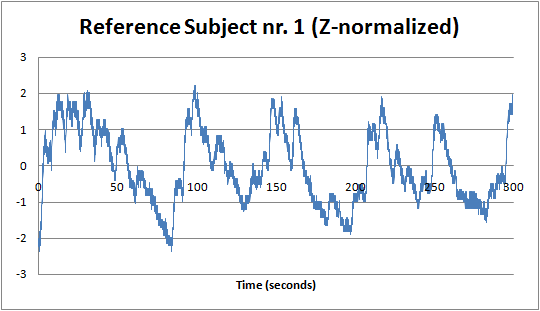
\includegraphics{ref1_ingela_r1_normalized.png}}
\caption{First reference subject, normalised EDA-value on y-axis.}
\end{figure}

\begin{figure}
\centerline{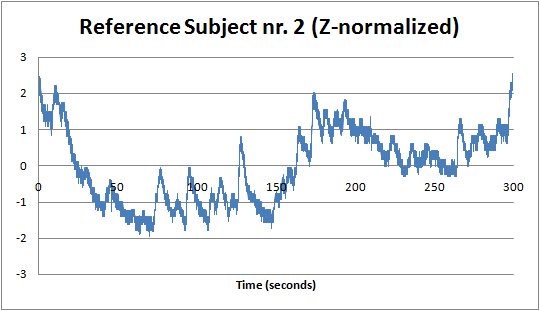
\includegraphics{ref2_henrik_r1_normalized.png}}
\caption{Second reference subject, normalised EDA-value on y-axis.}
\end{figure}
\vfill
\clearpage

\newpage
\vfill
\begin{figure}
\centerline{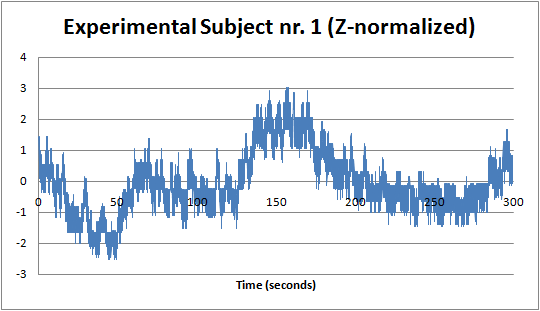
\includegraphics{exp1_rasmus_r1_normalized.png}}
\caption{First experimental subject, normalised EDA-value on y-axis.}
\end{figure}

\begin{figure}
\centerline{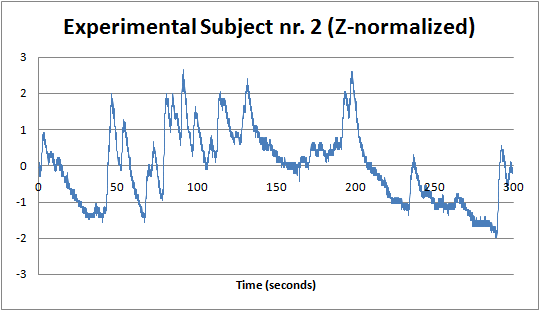
\includegraphics{exp2_my_r1_normalized.png}}
\caption{Second experimental subject, normalised EDA-value on y-axis.}
\end{figure}
\vfill
\clearpage

\newpage
\vfill
\begin{figure}
\centerline{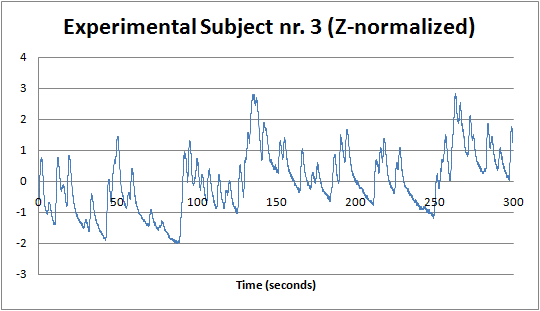
\includegraphics{exp3_peter_m_r1_normalized.png}}
\caption{Third experimental subject, normalised EDA-value on y-axis.}
\end{figure}

\begin{figure}
\centerline{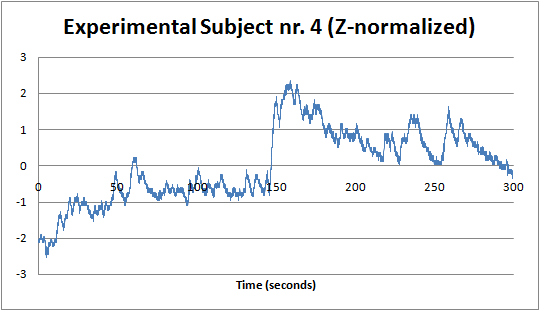
\includegraphics{exp4_peter_b_r1_normalized.png}}
\caption{Fourth experimental subject, normalised EDA-value on y-axis.}
\end{figure}
\vfill
\clearpage



\newpage
\vfill
\begin{figure}
\centerline{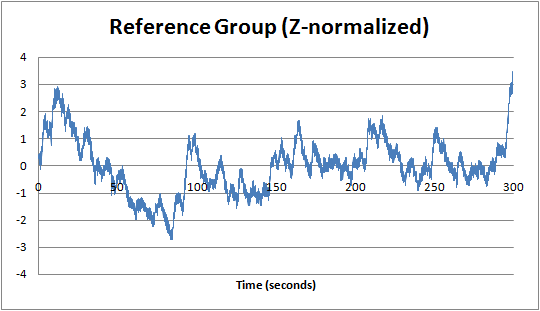
\includegraphics{ref_group_r1_normalized.png}}
\caption{Reference group results, normalised EDA-value on y-axis.}
\end{figure}

\begin{figure}
\centerline{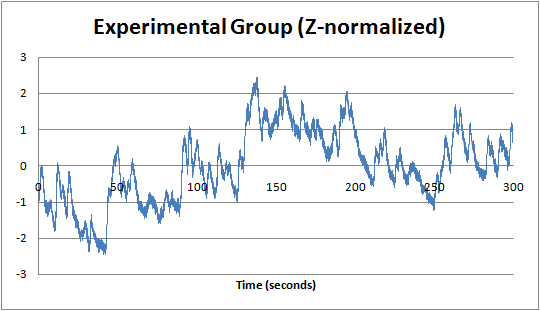
\includegraphics{exp_group_r1_normalized.png}}
\caption{Experimental group results, normalised EDA-value on y-axis.}
\end{figure}
\vfill
\clearpage

\section{Survey Results}
Following section presents results obtained from the survey that was handed out shortly after the user experiment had finished. Results are presented for each question in the survey, where the average value for each group is presented. An average value for the entire set of test subjects is also given. For questions in the survey that was asked to be filled with free text, results are given as a shorter summary. 

As already mentioned, graded questions were asked as statements on a scale from 1 to 4, where 1 corresponded to no conformity at all and 4 represented maximum conformity.

\begin{enumerate}
  \item I felt stress or arousal at some point during the play session. (Graded)  
  \begin{enumerate}
    \item All test subjects: 3.3
    \item Reference group: 3.0
	\item Experimental group: 3.5
  \end{enumerate}  
  \item At what time during the play session did you feel most arousal? (Free text)
  \\
  Result: Most people found themselves to become more stressed and aroused when the game speed got faster. One subject from the experimental group mentioned he became more stressed when given instructions to make the game go faster.
  \item I felt the game speed/game difficulty correlated with the grade of my stress or levels of emotional arousal. (Graded)
   \begin{enumerate}
    \item All test subjects: 2.0
    \item Reference group: 1.5
	\item Experimental group: 2.5
  \end{enumerate} 
  \item Did you feel that the game speed became faster or slower during periods of arousal? (Free text)
  \\
  Result: Almost all subjects stated they thought the game to speed up during moments of stress and arousal. One subject did not answer the question, and another felt the game to behave more randomly.
  \item I find the use of a biofeedback feature such as this made the game more enjoyable than usual. (Graded)
   \begin{enumerate}
    \item All test subjects: 2.9
    \item Reference group: 2.5
	\item Experimental group: 3.3
  \end{enumerate} 
  \item The game was more difficult to control with the EDA wristband equipped. (Graded)
   \begin{enumerate}
    \item All test subjects: 2.8
    \item Reference group: 3.0
	\item Experimental group: 2.5
  \end{enumerate} 
  \item I felt I could deliberately manipulate the game speed. (Graded)
   \begin{enumerate}
    \item All test subjects: 2.1
    \item Reference group: 1.5
	\item Experimental group: 2.8
  \end{enumerate} 
  \item Can you name other game titles you think would benefit by implementing biofeedback features such as this? (Free text) \\
  Result: Most test subjects mentioned other puzzle games; however some of them thought game titles in the horror, dance or first-person-shooter genres would also fit well.
  \item I am an experienced Tetris player. (Graded)
   \begin{enumerate}
    \item All test subjects: 3.4
    \item Reference group: 3.0
	\item Experimental group: 3.8
  \end{enumerate} 
\end{enumerate}
\chapter{Discussion}
In the following chapter we will look at some interesting parts of our results, in particular discuss similarities and oddities between what we have found in the results of the user experiment and the survey. One interesting question in particular that relates close to the problem statement of this thesis is that of question number seven in the survey: "I felt that I could deliberately manipulate the speed of the game". We will look at the experimental results for some subjects and compare their survey answers to the experimental results in order to investigate if there was any resemblance to the answer of this question and the actual result.

We will also look into other topics of interest, such as possible usage of EDA in different video game titles, difficulties with the project overall, compare the actual results to what we previously had expected of the project and also make some suggestions for future studies on the subject.

\section{Discussion of Survey and Experimental Results}
The highest peak in the experimental group's summarised plots (Figure 4.8) lies around the 135 second mark. This shows that there was some activity after we told the subjects to try to make the game go faster. However after the 3 minute mark when we told them to try to calm down and make the game go slower we could identify another peak, then mostly a downwards slope. Even at the last instruction (4 minute mark), where we told the subjects to take a deep breath and calm down, a third peak shows. These are the three highest peaks in the plot.

The same pattern shows on most of the individual plots from each experimental subject when looking at the different minute marks. Looking at the reference group's summarised plots (Figure 4.7.) and individual plots (Figure 4.1. - 4.2.) the measurements are more random. We can see no common pattern.

Even though the reference group played a second round after we had explained how the game and the sensor worked, and what the actual experiment was about, comparing both group averages on the survey shows that the experimental group both felt like the game speed correlated with their stress/arousal and that they deliberately could manipulate the game speed more than the reference group who had not been given any instructions.

It seems like it is easier to consciously raise the value than lowering it. Focusing on calming down and lowering the value might actually raise the cognitive activity and create a peak. However continuous calming might lower the average in the long run.

\section{Usage of EDA in Different Games}
One interesting aspect of the survey results we found was that most subjects thought the EDA implementation we made of Tetris to be more fun and engaging than a regular version of the game. This opens up the question however other games could benefit from using EDA biofeedback. Again looking at the survey results, we find that most test subjects thought that usage of a similar wristband would be well suited in other puzzle games with difficulty aspects of time and speed variations. Other titles mentioned from the survey were horror games and FPS-titles.

One game we immediately began to think of is the Swedish independent survival horror game Amnesia: The Dark Descent \cite{amnesia}. Amnesia is an FPS-title with unique horror elements developed by Frictional Games, a game very well received that has won numerous awards. One part of the game's mechanics is a "sanity-level" that measures a player's emotional stability. When confronted by scary or horrific elements during progress, the sanity-level goes down and vision becomes blurred. The game character's environment may become distorted, and other psychedelic effects arise in order for the player to become more afraid and confused. As for now, these "sanity effects" are heavily scripted into the game, and we think the use of EDA biofeedback in games with similar mechanics could prove to be very interesting.
\section{Difficulties}
We realise that posing the question whether one may alter live EDA measurements during computer gaming or not requires thorough user experiments with a large number of test participants. Another aspect that would be required is to analyse result data in a statistical way, such as issuing standardised z-score tests between group populations in order to verify differences. One of the greatest difficulties during this project was how to represent and analyse the experimental result data. Time constraints forced us to only plot the data and make a more general discussion about how the plots differed between groups and also how the experimental data correlated to answers made in the survey. A more thorough approach would be to make statistical tests and compare specific time frames where subjects were asked to fasten or lower game speed; however the small amount of test subjects we were able to gather and lack of time forced us to only look at the data and make very general and non-statistical conclusions. Another difficulty was how to actually implement the biofeedback feature in the game; in a more thorough project one could argue that several game versions that behave differently would be required to produce more convincing results.

\section{Expected Results}
Our final result was in some terms what we had hoped to achieve before we started this project. However, when reflecting back on the span of the project we had hoped to get more convincing and accurate results, and also be able to present them in a more correct and convincing manner. We were not able to produce a convincing answer to our problem statement, such as "It is possible to do this", but rather only make very general conclusions by looking at the little data we got.

We only got vague conclusions of our problem statement, however the project itself was a very rewarding experience for us since it involved many different aspects of what we strive to learn and become better at. To use the Q-Sensor in a larger project was interesting, and it was a fun challenge to implement biofeedback features in a video game since we have done nothing similar to this in the past.

\section{Suggestions for Further Research}
First and foremost a much larger study is needed in order to produce more convincing results. A similar study to this one, with more aspects of game mechanics, larger test groups, and statistical analysis of data between groups is needed to be able to arrive at more convincing conclusions. Also, the use of different games other than just one (in our case, Tetris) would be recommended. It would be interesting to see if results differed between groups playing a simple puzzle game similar to Tetris and other groups playing more complex ones, such as horror titles.

\chapter{Conclusions}
To answer whether it is possible to alter live measurements of EDA during biofeedback gaming proved to be a more difficult question than we first thought. With the result we obtained from our user experiment we could see that there surely happens something when subjects are instructed to change biofeedback elements in our Tetris version. However, to actually prove any results, one needs to issue a similar research project with much larger test groups and analyse and represent data in a more statistical manner.

From the small experiment we have done there is certainly a possibility that one can manipulate the EDA value deliberately, but not control it very precisely. One might get a reaction in measurements but it will not always be the reaction aimed for.

\begin{thebibliography}{9}

\bibitem{driving}
  Schnittker,
  \emph{Electrodermal Activity of Novice Drivers During Driving Simulator Training}.
  University of Twente,
  2012

  \bibitem{fps}
  Kuikkaniemi et al.
  \emph{The influence of implicit and explicit biofeedback in first-person shooter games}.
  ACM New York, NY, USA,
  2010
  
  \bibitem{tetris10}
  Guillaume et al.
  \emph{GamEMO: how physiological signals show your emotions and enhance your game experience}.
  ACM New York, NY, USA,
  2012
  
  \bibitem{affectiva}
  Affectiva website,
  \emph{Understanding EDA}.
  http://www.affectiva.com/q-sensor/resources/understanding-eda/,
  Visited 2013-03-20
  
  \bibitem{sics}
  SICS website,
  \emph{Affective Health Project}.
  https://www.sics.se/projects/affective-health,
  Visited 2013-04-02
  
  \bibitem{code}
  Google Code,
  \emph{Java Source Code for Tetris implementation}.
  http://tinyurl.com/c9une7g,
  Visited 2013-03-15
 
 \bibitem{r}
  RXTX Website,
  \emph{RXTX Library}.
  http://RXTX.qbang.org/wiki/index.php/FAQ,
  Visited 2013-03-20
  
  \bibitem{amnesia}
  Amnesia Website,
  \emph{The Amnesia Game}.
  http://www.amnesiagame.com/
  Visited 2013-04-05
  
  \bibitem{excel}
  Shawn McClain, Demand Media,
  \emph{How to Normalize in Excel}.
  http://smallbusiness.chron.com/normalize-excel-36009.html
  Visited 2013-04-03
  
\end{thebibliography}

\appendix
\addappheadtotoc
\chapter{Java Source Code}\label{appA}
\section{PortReader class}
Class available online at http://pastie.org/7466097 
\section{Tetris class}
Class available online at http://pastie.org/7465977
\end{document}
